\section{Evaluation}\label{sec:evaluation}

To evaluate the performances of our approach, we first evaluate its  raw speed with a test class that we made for the occasion. We also ran two series of tests: we first tested all classes in \texttt{java.lang} $10^{6}$ times each. We also tested a package from iText\footnote{http://www.lowagie.com/iText/ downloaded Sep. 1, 2009} a well known library -- 1,969,220 downloads on SourceForge\footnote{http://sourceforge.net/projects/itext/}, $84\%$ positive advices, activity of $99.85\%$ -- for manipulating PDF documents in Java. 

All tests were run using a MacBook Pro 2.53 GHz Intel Core 2 Duo, 4GB of 1067 MHz DDR3 of RAM, under MacOSX with the Java(TM) SE Runtime Environment (build 1.6.0\_15-b03-219) -- with default value of 64MB of RAM reserved. 

\subsection{Performances}

To test raw performances of YETI, we made two small classes -- \texttt{Perf} and \texttt{Perf1} shown in Figure~\ref{fig:perf} -- that we tested 30 times each with one million tests. Results are presented in Figures~\ref{fig:perfDriver} and~\ref{fig:perfValue}.

\begin{figure}[h!]
{\small
\begin{verbatim}
public class Perf{
        int i=0;
        public void test(){
                i++;
        }
}
public class Perf1{
        public void test(int i){
                int j = i;
                i++;
                assert(i>j);
        }
}
\end{verbatim}
}
\caption{Classes used for measuring performances.}\label{fig:perf}
\end{figure}

While \texttt{Perf} does not exhibit failures, \texttt{Perf1} exhibits failures when \texttt{i} is equal to \texttt{MAX\_INT} if assertions are enabled (which we chose to do in this test).

\begin{figure}[h!]
\begin{center}
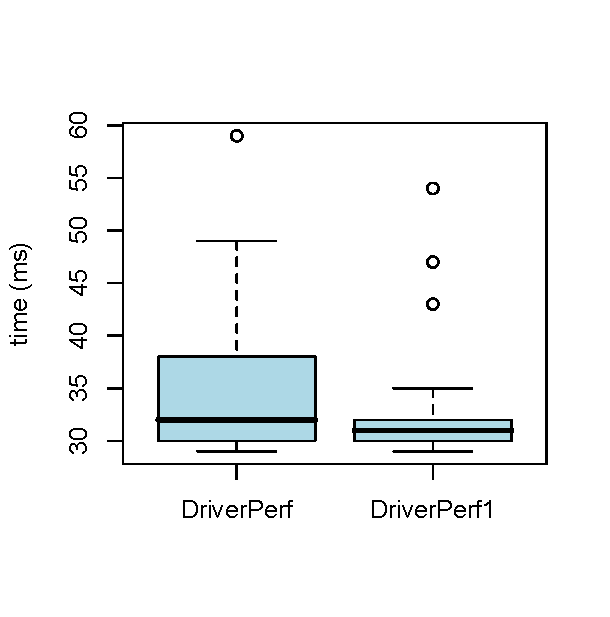
\includegraphics[width=6cm]{images/DriverWhiskers.pdf}
\end{center}
\caption{Evaluation of the code of Perf and Perf1 with an external driver.}\label{fig:perfDriver}
\end{figure}

To make sure that we only tested the overhead of the infrastructure, we also made one million calls on each of the methods from another program. Figure~\ref{fig:perfDriver} shows box and whisker plots for the two raw tests.

\begin{figure}[h!]
\begin{center}
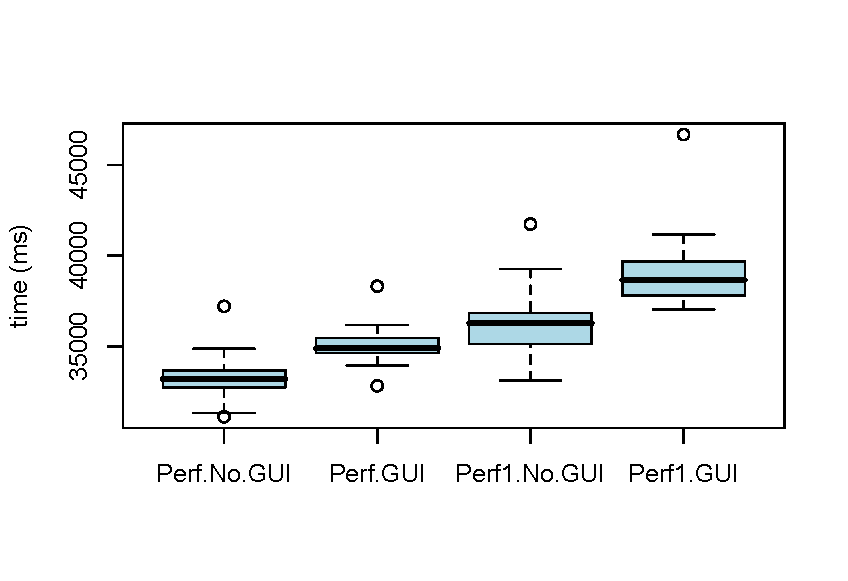
\includegraphics[width=9cm]{images/PerfWhiskers.pdf}
\end{center}
\caption{Evaluation of the code of Perf and Perf1 tested by YETI, with and without GUI. Averages: 33200(Perf No GUI), 35018(Perf GUI), 36103(Perf1 No GUI), 39021(Perf1 GUI)}\label{fig:perfValue}
\end{figure}

Figure~\ref{fig:perfValue} shows box and whisker plots for 30 YETI testing sessions of one million tests made on \texttt{Perf} and \texttt{Perf1}, both with and without the GUI. We can see that there is a slowdown of more than a factor 1000 over the direct invocation. The GUI also incurs respectively a $5.5\%$ and $8.1\%$ overhead.



\subsection{Testing \texttt{java.lang}}

\begin{table}[h!]
\caption{Results of testing java.lang}\label{tab:javalang}
\begin{center}
\begin{tabular}{l c c c c c c c c}
\hline
&\begin{sideways}Total throwables\end{sideways}&\begin{sideways}Faults\end{sideways}&\begin{sideways}NullPointer\end{sideways}&\begin{sideways}NoClassDefFoundError\end{sideways}&\begin{sideways}IndexOutOfBounds\end{sideways}&\begin{sideways}AssertionError\end{sideways}&\begin{sideways}IllegalArgument\end{sideways}\\
\hline
Boolean &1&0&0&&&&\\
Byte &2&2&2&&&&\\
Character &33&1&1&&&&\\
Character.Subset &0&0&&&&&\\
Character.UnicodeBlock &2&0&&&&&\\
Class &13&3&3&&&&\\
ClassLoader &10&10&8&2&&&\\
Compiler &0&0&&&&&\\
Double &4&2&2&&&&\\
Enum &2&0&&&&&\\
Float &4&2&2&&&&\\
InheritableThreadLocal &0&&&&&&\\
Integer &2&2&2&&&&\\
Long &2&2&2&&&&\\
Math &0&&&&&&\\
Number &0&&&&&&\\
Object &0&&&&&&\\
Package &1&1&1&&&&\\
Process &0&&&&&&\\
ProcessBuilder &5&2&2&&&&\\
Runtime &2&0&&&&&\\
RuntimePermission &4&0&&&&&\\
SecurityManager &39&0&&&&&\\
Short &2&2&2&&&&\\
StackTraceElement &2&0&&&&&\\
StrictMath &0&&&&&&\\
String &87&5&&&2&3&\\
StringBuffer &57&3&&&2&&1\\
StringBuilder &36&2&1&&&&1\\
System &5&0&&&&&\\
Thread &18&5&5&&&&\\
ThreadGroup &4&0&&&&&\\
ThreadLocal &0&&&&&&\\
Throwable &2&0&&&&&\\
Void&0&&&&&&\\
EnumConstantNotPresentException&1&1&1&&&&\\
All Other Exceptions  &0&0&0&&&&\\
All Errors  &0&0&0&&&&\\
\hline
Total&340&45&34&2&4&3&2\\
\hline
Percentages&&&75.6&4.4&8.9&6.7&4.4\\
\hline
\end{tabular}
\end{center}
\end{table}

We tested all classes in \texttt{java.lang} with YETI. For each class we requested $1,000,000$ tests. Except for a couple of classes that were too memory intensive --�such as \texttt{StringBuffer} -- that we tested with $100,000$ tests only.
Table~\ref{tab:javalang} shows our results. The first column of numbers indicates the total number of
throwables that the tests triggered. We then classified each throwable as either a fault or not. This is due to programmers not necessarily declaring runtime exceptions but rather indicating in the documentation that these exceptions are normal. For throwables that where not ruled out, 
we then classify them by column. Note that the documentation of certain classes states up front that
some kind of exceptions are to be expected -- for example \texttt{NullPointerException} in \texttt{String}.
Other classes declare all runtime exceptions. This indicates that several teams actually collaborated to make this API. 

The small number of faults other than \texttt{NullPointerException}s, shows the overall quality of \texttt{java.lang} in terms of API and implementation. Most exception seem indeed to be omitted in the documentation rather than real bugs in the system.

It is however compelling to see that YETI can actually uncover 45 faults in a library as used and tested as \texttt{java.lang}. To obtain more data to assess how useful YETI would be for regular developers, we present similar results for a regular open source project in the next section.



\subsection{Testing \texttt{com.lowagie.text} from iText}

\begin{table}[h!]
\caption{Results of testing com.lowagie.text}\label{tab:comlowagietext}
\begin{center}
\begin{tabular}{l c c c c c c c c c c c c c c c}
\hline
&\begin{sideways}Total throwables\end{sideways}&\begin{sideways}Number of Faults\end{sideways}&\begin{sideways}NullPointer\end{sideways}&\begin{sideways}IndexOutOfBounds\end{sideways}&\begin{sideways}NumberFormatException\end{sideways}&\begin{sideways}IllegalArgumentException\end{sideways}&\begin{sideways}No class def found\end{sideways}&\begin{sideways}ClassCast\end{sideways}&\begin{sideways}IllegalState\end{sideways}&\begin{sideways}NegativeArraySize\end{sideways}&\begin{sideways}Runtime\end{sideways}&\begin{sideways}ArrayStore\end{sideways}&\begin{sideways}StackOverflow\end{sideways}&\begin{sideways}Project-defined\end{sideways}\\
\hline
Anchor &&&&&&&&&&&&&&\\
Annotation &1&1&1&&&&&&&&&&&\\
Cell &20&5&2&&2&1&&&&&&&&\\
Chapter &&&&&&&&&&&&&&\\
ChapterAutoNumber &&&&&&&&&&&&&&\\
Chunk &3&3&1&&&1&1&&&&&&&\\
Document &18&18&4&&&&&&&&&&2&12\\
DocWriter &&&&&&&&&&&&&&\\
ElementTags &&&&&&&&&&&&&&\\
Font &3&3&1&&&&2&&&&&&&\\
FontFactory &4&4&3&&&&&&&&&&&1\\
FontFactoryImp &1&1&&&&&&&&&&&&1\\
GreekList &&&&&&&&&&&&&&\\
Header &&&&&&&&&&&&&&\\
HeaderFooter &&&&&&&&&&&&&&\\
Image &4&4&3&1&&&&&&&\\
ImgCCITT &&&&&&&&&&&\\
ImgJBIG2 &1&1&1&&&&&&&&\\
ImgRaw &&&&&&&&&&&\\
ImgTemplate &&&&&&&&&&&\\
ImgWMF &2&2&2&&&&&&&&\\
Jpeg &2&2&2&&&&&&&&\\
Jpeg2000 &2&2&2&&&&&&&&\\
List &1&1&1&&&&&&&&\\
ListItem &3&3&1&&&&1&1&&&\\
MarkedObject &1&1&1&&&&&&&&\\
MarkedSection &4&3&2&1&&&&&&&\\
Meta &2&2&2&&&&&&&&\\
PageSize &1&1&&&&&&&&&1\\
Paragraph &2&2&&&&&&2&&&\\
Phrase &4&4&2&1&&&&1&&&\\
Rectangle &3&3&2&&&&&&&&&&&1\\
RectangleReadOnly &17&17&&&&&&&&&&&&17\\
RomanList &1&1&&&&&1&&&&&&&\\
Row &&&&&&&&&&&&&&\\
Section &6&3&&2&&&&&1&&&&&\\
SimpleCell &1&1&&&&&&&&&&&&1\\
SimpleTable &1&1&&&&1&&&&&&&&\\
SpecialSymbol &&&&&&&&&&&&&&\\
Table &26&26&3&13&&2&1&&&6&&2&&\\
Utilities &4&4&2&2&&&&&&&&&&\\
ZapfDingbatsList &&&&&&&&&&&&&&\\
ZapfDingbatsNumberList&&&&&&&&&&&&&&\\
All Exceptions&&&&&&&&&&&&&&\\
\hline
Total&138&120&38&20&2&5&6&4&1&6&1&2&2&33\\
\hline
Percentage&&86.2&31.9&16.8&1.7&4.2&5.0&3.4&0.8&5.0&0.8&1.7&1.7&27.7\\
\hline
\end{tabular}
\end{center}
\end{table}

In order to have a more representative project for end-users, we tested the package \texttt{com.lowagie.text} from iText. Because this package is quite time intensive to test, we decided to test all classes in the package at the same time for only a $100000$ tests. The testing session lasted for 15 minutes and output 138 unique failures. Comparatively to the previous section, the code almost did not declare any runtime exception. Only five classes --~\texttt{Cell}, \texttt{MarkedSection}, \texttt{Phrase}, \texttt{RectangleReadOnly}, and \texttt{Section}~-- did it in an informal way. 

It is worth noting that two classes --~\texttt{RectangleReadOnly}  and \texttt{Document}~-- exhibit a high number of project-defined errors. We investigated and found out that these two classes have poor documentation rather than poor code. This is to be expected in a free open source project as the code often serves as documentation.

Eventually, even over long running sessions (when logs are not stored within YETI) the number of routine calls effected, grows linearly with time as shown in Figure~\ref{fig:string} for a 50 minute session testing \texttt{java.lang.String}.

\begin{figure}[h!]
\begin{center}
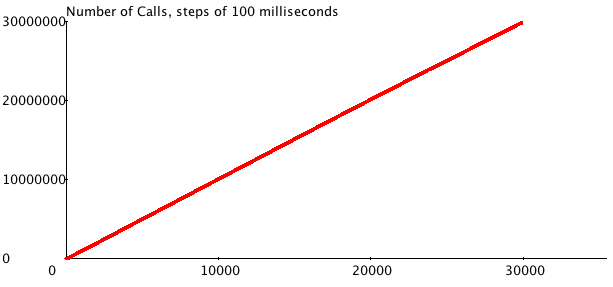
\includegraphics[width=10cm]{images/Ncalls.png}
\end{center}
\caption{Number of calls over time while testing \texttt{java.lang.String}}\label{fig:string}
\end{figure}

